% Deriving  a policy
\section{Deriving a policy}\label{subsec:Deriving a policy}
%Our focus is on the former, learning low-level trajectories that can be generalised.
%The latter will then be taken over by automated planning techniques.

Once the dataset of examples has been acquired, the robot learner needs to derive a policy $\pi : Z \rightarrow A$, a state-action mapping from the observed state to the action domain representing the desired behaviour. 
\cite{chernova2014robot} give an overview of the state of the art policy derivation techniques.
The most efficient ones approximate the state-action mapping from as few training examples as possible.
PbD can be classified into low-level skill learning (trajectory encoding) and high-level task learning (symbolic encoding).
Low-level representations focus on learning generalised trajectories from the human demonstrator, high-level representations focus on learning a sequence of motion elements (primitives) (\cite{peppoloni2014ros}). In the following we will give an overview of both techniques.


\subsection{Low-level skill learning}
In the literature low-level actions have been referred to as \textit{skill, motor skill, primitive action,} or \textit{low-level motion} (\cite{chernova2014robot}).
Generalisable low-level actions can be learned by recording joint angle trajectories using GMM (\cite{billard2008robot}), using keyframe-based learning (\cite{akgun2012keyframe}), or using Dynamic Movement Primitives (DMP) (\cite{pastor2009learning}), which consist of differential equations that can create a smooth trajectory to a new goal point.

For instance, in keyframe-based learning, demonstrations are provided by kinesthetically manipulating the robot's arm and recording a series of end-effector positions (or \textit{keyframes}). 
An end-effector pose can be relative to the robot's base or to a landmark previously detected by the robot.
Landmarks are only known to the robot after a table top detection step has been performed.

\begin{table}[ht]
\centering
\caption{Task representations}
\label{tab:representations}
\begin{tabular}{r|ll}
 & Continuous representation & Symbolic representation\\ \hline
Position & (x,y,z) coordinates & table \\
Orientation  & Theta x,y,z  & straight/upright \\
Colour & (r,g,b) & Red, yellow, green ranges\\
Spatial preposition between 2 objects & (x,y) distance vector & Left/right/front/behind of 
\end{tabular}
\end{table}

\subsection{High-level task learning}
For learning high-level tasks it is assumed that a set of low-level primitive actions is preprogrammed into the robot. 
\cite{she2014teaching} teaches the robot new high-level actions by instructing the robot a sequence of lower-level actions.
Rather than representing the new action as an action sequence, it is modelled by their desired goal states calculated as:
$A_i(c_1 \dots c_k) = (S_e - S_e \cap S_b) \cup p_{grip}$ where $c_i$ are objects in the scene, $S_b$ and $S_e$ are the states at the beginning and end of the instruction and $p_{grip} = \{open, close\}$ is the gripper status at the end of instruction.
As the work uses the blocks world domain with a single object type (`block'), an operator for the new high-level action can be inferred easily. Preconditions and effects for the domain are already specified in advance.

Figure \ref{fig:Learning-techniques} shows a categorisation of policy derivation techniques, which can be split into three main approaches: Mapping functions, system models, and plans.

% \#TO DO: add User intentions, Policy derivation Planner
\begin{figure}[!h]
	\centering
	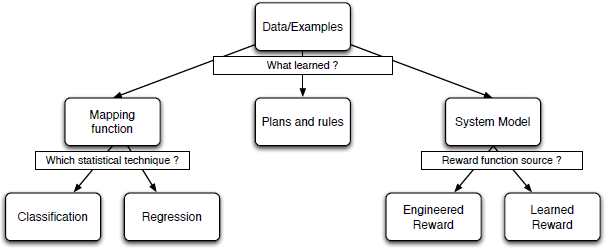
\includegraphics[scale=0.75]{figures/Learning-techniques}
	\caption{Policy derivation techniques (\cite{argall2009survey})}
	\label{fig:Learning-techniques}
\end{figure}


\subsubsection{Mapping function} 
A function is calculated that approximates the state-to-action mapping $f : Z \rightarrow A$ for the demonstrated behaviour. The function approximation technique depends on the learning technique, i.e. whether the robot learner is provided with the data incrementally or once all data has been gathered. Mapping approximation techniques are generally split into two categories, depending on the continuity of the prediction output, whether they are produced as discrete states (\textit{Classification}) or continuous values (\textit{Regression}) (\cite{argall2009survey}).

Classification techniques categorise their input and output into discrete classes, grouping similar input values together. One classification algorithm can be applied to varying action control levels, from basic motion control to complex behaviours. Techniques are used in combination with other classifiers such as k-Nearest Neighbours (kNN) to learn navigation behaviours (\cite{saunders2006teaching}), or Hidden Markov Models (\cite{hovland1996skill}) to learn motion primitives (\cite{rybski1999interactive}).

Regression techniques map demonstration states to continuous action spaces, with the robot actions being a continuous output. These algorithms are typically applied to low-level motions, as the continuous-valued output often results from combining actions from multiple demonstration sets. Regression techniques are distinguished between whether the function approximation occurs at run time, e.g. using a Lazy Learning technique (\cite{atkeson1997locally}), such as kNN for action selection, or prior to run time, e.g. using Neural Networks, to enable autonomous driving (\cite{pomerleau1991efficient}).

\subsubsection{System models}
A state transition model of the world $T(s'|s, a)$ and a reward function $R(s)$ are determined for different states $s$ from the demonstration data, which are then used to learn a policy $\pi : Z \rightarrow A$. With the goal to maximise the cumulative reward over time, the reward function can either be user-defined or learned from demonstration data.
User-defined, or \textit{engineered} reward functions often rely on demonstration-based techniques in order to highlight interesting areas of the state space and eliminate long periods of initial exploration, that may acquire no reward feedback (\cite{smart2002effective}).
On the other hand, reward functions can be learned by rewarding higher similarity for states already encountered during demonstrations (\cite{atkeson1997robot}), or for well-estimated trajectories and features (\cite{abbeel2004apprenticeship}).
